\begin{enumerate}[label=\thechapter.\arabic*,ref=\thechapter.\theenumi]
\item
For the circuit given below, choose the angular frequency $ \omega_0$ at which voltage across capacitor has maximum amplitude?
\begin{figure}[h!]
    \includegraphics[width = 0.5\columnwidth]{2023/BM/16/figs/c_fig1.pdf}
    \caption{circuit }
    \centering
    \label{fig: bm_16_fig_1}
\end{figure}
\begin{enumerate}
    \item[(A)] 1000
    \item[(B)] 100
    \item[(C)] 1
    \item[(D)] 0   
\end{enumerate}
\hfill(GATE BM 2023 Question 16)\\

\solution
\input{2023/BM/16/asnmt3.tex}
\newpage
\item
In the following circuit, the switch S is open for $t < 0$ and closed for $t \ge 0$.
What is the steady state voltage (in Volts) across the capacitor when the switch is closed?
\begin{figure}[h!]
    \includegraphics[width = 0.7\columnwidth]{2023/BM/30/figs/c_fig1.pdf}
    \caption{circuit }
    \centering
    \label{fig:bm_30_fig_1}
\end{figure}
\hfill(GATE BM 2023 Question 30) \\
\solution
\iffalse
\let\negmedspace\undefined
\let\negthickspace\undefined
\documentclass[journal,12pt,twocolumn]{IEEEtran}
\usepackage{cite}
\usepackage{amsmath,amssymb,amsfonts,amsthm}
\usepackage{algorithmic}
\usepackage{graphicx}
\usepackage{textcomp}
\usepackage{xcolor}
\usepackage{txfonts}
\usepackage{listings}
\usepackage{enumitem}
\usepackage{mathtools}
\usepackage{gensymb}
\usepackage{comment}
\usepackage[breaklinks=true]{hyperref}
\usepackage{tkz-euclide}
\usepackage{listings}
\usepackage{gvv}
\def\inputGnumericTable{}
\usepackage[latin1]{inputenc}
\usepackage{color}
\usepackage{array}
\usepackage{longtable}
\usepackage{calc}
\usepackage{multirow}
\usepackage{hhline}
\usepackage{ifthen}
\usepackage{lscape}

\newtheorem{theorem}{Theorem}[section]
\newtheorem{problem}{Problem}
\newtheorem{proposition}{Proposition}[section]
\newtheorem{lemma}{Lemma}[section]
\newtheorem{corollary}[theorem]{Corollary}
\newtheorem{example}{Example}[section]
\newtheorem{definition}[problem]{Definition}
\newcommand{\BEQA}{\begin{eqnarray}}
\newcommand{\EEQA}{\end{eqnarray}}
\newcommand{\define}{\stackrel{\triangle}{=}}
\theoremstyle{remark}
\newtheorem{rem}{Remark}
\begin{document}

\bibliographystyle{IEEEtran}
\vspace{3cm}

\title{GATE 2023 BM 30}
\author{EE23BTECH11007 - Aneesh Kadiyala$^{*}$% <-this % stops a space
}
\maketitle
\newpage
\bigskip

\renewcommand{\thefigure}{\theenumi}
\renewcommand{\thetable}{\theenumi}

\vspace{3cm}
\textbf{Question:} In the following circuit, the switch S is open for $t < 0$ and closed for $t \ge 0$.
What is the steady state voltage (in Volts) across the capacitor when the switch is closed?
\begin{figure}[h!]
    \centering
    \includegraphics[width = \columnwidth]{2023/BM/30/figs/c_fig1.pdf}
\end{figure}
\\
\solution
\\
\fi
\begin{figure}[h!]
    \centering
    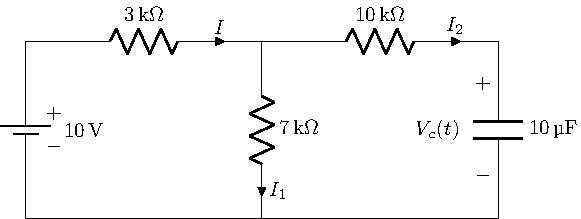
\includegraphics[width=\columnwidth]{2023/BM/30/figs/c_fig3.pdf}
\end{figure}
\\
In steady state, no current flows through the capacitor.
\begin{align}
I_2 &= 0 \\
V_c &= \brak{7\text{k}\ohm}I_1 \\
&= \brak{7\text{k}\ohm}I \\
&= \brak{7\text{k}\ohm}\frac{10\text{V}}{10\text{k}\ohm} \\
\implies V_c &= 7\text{V}
\end{align}
In s-domain:
\begin{figure}[h!]
    \centering
    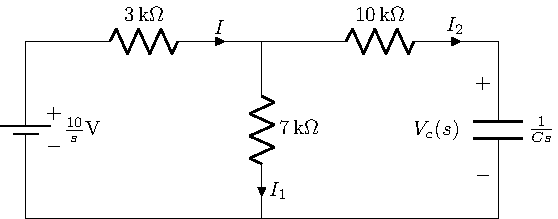
\includegraphics[width=\columnwidth]{2023/BM/30/figs/c_fig2.pdf}
\end{figure}
\begin{align}
\implies I\brak{s} &= \frac{\frac{10}{s}\text{V}}{3\text{k}\ohm + \frac{(7\text{k}\ohm)(10\text{k}\ohm + \frac{1}{sC})}{17\text{k}\ohm + \frac{1}{sC}}} \\
I &= I_1 + I_2 \\
I_1\brak{7\text{k}\ohm} &= I_2\brak{10\text{k}\ohm + \frac{1}{sC}} \\
I_2\brak{s} &= \frac{7\text{k}\ohm}{17\text{k}\ohm + \frac{1}{sC}}I\brak{s} \\
%&= \frac{\frac{70000}{s}}{121 * 10^6 + \frac{10000}{sC}} \\
%&= \frac{\frac{7}{s}}{121 * 10^2 + \frac{1}{sC}} \\
\implies I_2\brak{s} &= \frac{7\brak{10^{-5}}}{0.121s + 1} \\
V_c\brak{s} &= I_2\brak{s}\frac{1}{sC} \\
&= \frac{7}{s\brak{0.121s + 1}} \\
%&= 7\brak{\frac{\frac{1}{0.121}}{s\brak{s + \frac{1}{0.121}}}} \\
&= 7\brak{\frac{1}{s} - \frac{1}{s + \frac{1}{0.121}}}
\end{align}
Taking inverse Laplace transform:
\begin{align}
V_c\brak{t} &= 7u\brak{t}\brak{1 - e^{-\frac{t}{-0.121}}} \label{eq:2023BM30}
\end{align}
\begin{figure}[h!]
\centering
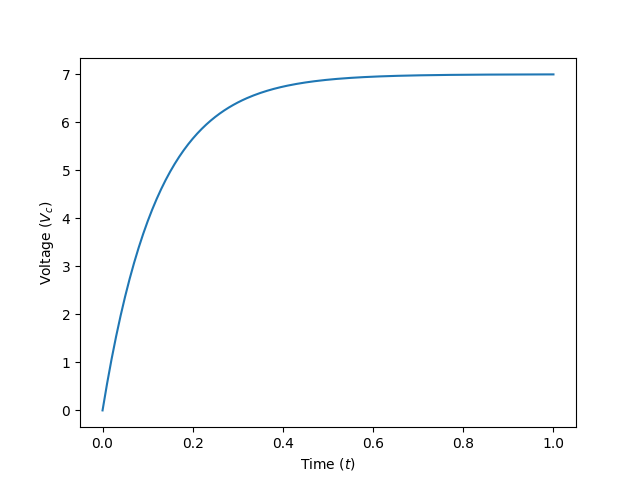
\includegraphics[width=\columnwidth]{2023/BM/30/figs/plot.png}
%\caption{$V_c$ vs $t$}
\label{fig:2023BM30}
\end{figure}
\\
In steady state $t \to \infty$. From \eqref{eq:2023BM30}:
\begin{align}
\lim_{t\to\infty}V_c\brak{t} &= 7\text{V}
\end{align}

\pagebreak
\item 
A finite impulse response (FIR) filter has only two non-zero samples in its impulse response $h[n]$, namely $h[0] = h[1] = 1$. The Discrete Time Fourier Transform (DTFT) of $h[n]$ equals $H(e^{j\omega})$, as a function of the normalized angular frequency $\omega$. For the range $\abs{\omega} \leq \pi$, $\abs{H(e^{j\omega})}$ is equal to
\begin{enumerate}
	\item[(A)] $2\abs{\cos(\omega)}$
	\item[(B)] $2\abs{\sin(\omega)}$
	\item[(C)] $2\abs{\cos(\frac{\omega}{2})}$
	\item[(D)] $2\abs{\sin(\frac{\omega}{2})}$
\end{enumerate}
\hfill(GATE BM 2023 Question 17) \\
\solution
\input{2023/BM/17/1.tex}
\pagebreak
\item
For the circuit shown,if $i=\sin 1000t$, the instantaneous value of the Thevenin's voltage(in volts) across the terminals a anb b at time t=5ms is\\[2pt]

\begin{circuitikz}[american voltages,american currents]
    % Draw the circuit components
    \draw (0,0) -- (2,0);
    \draw (2,2) to [resistor,l=$10\Omega$] (2,4);
    \draw (2,4) -- (0,4);
    \draw (2,0) to [capacitor,l=$-j10\Omega$,-,i_=$i_x$] (2,2);
    \draw (2,0) -- (5,0);
    \draw (5,0) to[inductor,l=$j10\Omega$] (5,2);
    \draw (5,2) to [resistor,l=$10\Omega$] (5,4);
  \draw (5,4) to [cV,l^=$4i_x$,invert] (2,4);
  \draw (5,4) -- (6,4);
  \draw (6,4) to[I,l=$\sin 1000t$,invert] (6,0);
  \draw (6,0) -- (5,0);
   \node[circle,fill=black,inner sep=1.5pt,label=above:a] at (0,0) {};
    \node[circle,fill=black,inner sep=1.5pt,label=above:b] at (0,4) {};
    \end{circuitikz}
    \hfill(GATE EE 2023 ) \\
    \solution
    \input{2023/EE/51/gate51.2023.tex}
    \pagebreak

    \item In the circuit shown ,$\omega=100\pi\text{rads/s}$, R1=R2=$2.2\Omega$ and L=$7\text{mH}$. the capacitance $\text{C}$ for which $Y_{in}$ is purely real is  $\text{mF}$ \\
	\begin{center}
	\begin{circuitikz} \centering \draw 
		(0,4) to[sinusoidal voltage source, l=$V_{0}$cos($\omega$t)] (0,0)
		(0,4) to[short] (4,4)
		(4,4) to[resistor, l=$R_1$ ] (4,2)
		(4,2) to[inductor, l= $\text{L} $] (4,0) to[short ] (0,0)
		(8,4)  to[short] (4,4)
		(8,4) to[resistor, l= $R_2$] (8,2) to[capacitor,l=$\text{C}$] (8,0) to (4,0);
	\end{circuitikz}
	\end{center}
\hfill(GATE IN 2023 Q46)\\
\solution
\input{2023/IN/46/7.tex}

\pagebreak
\item An input voltage in the form of a square wave of frequency $1\, kHz$ is given to a circuit, which results in the output shown schematically below. Which one of the following options is the CORRECT representation of the circuit? \hfill(GATE PH 2023 Q37)
\begin{figure}[!h]
    \centering
    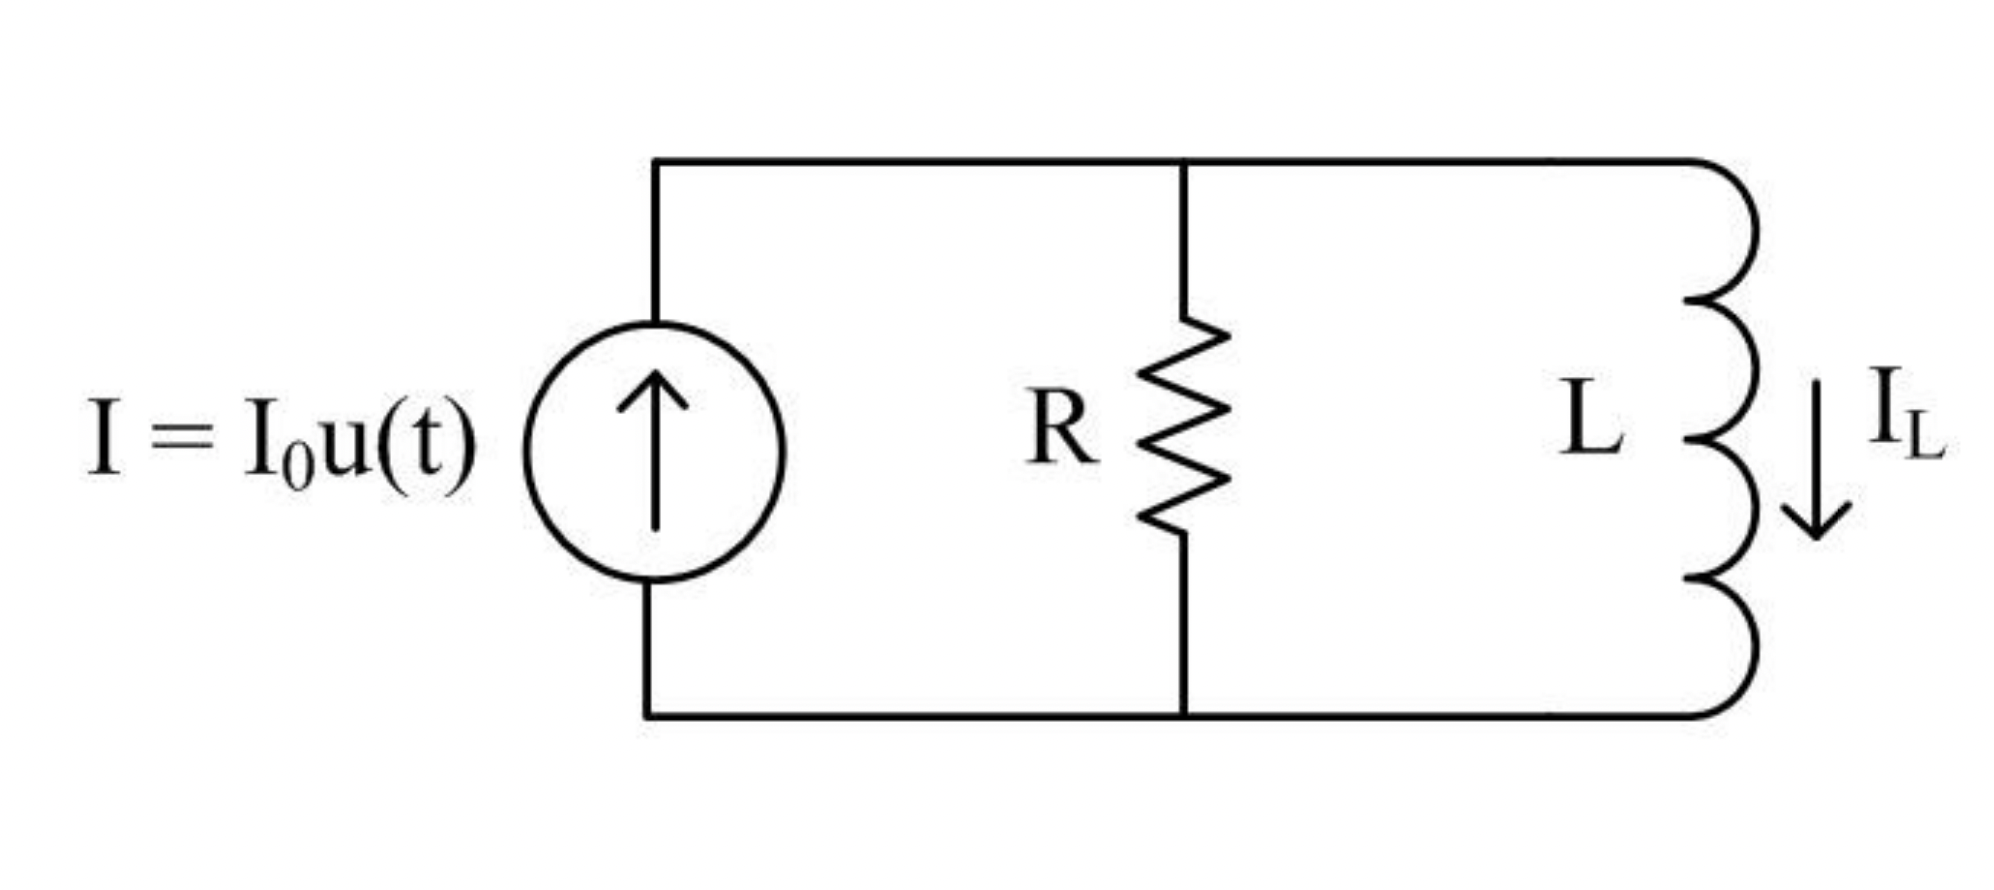
\includegraphics[width = 0.6\columnwidth]{2023/PH/37/figs/question.png}
	\caption{}\
	\label{fig:ques_gate.ph.23.37}
\end{figure}

\begin{enumerate}[label = (\alph*)]
    \item 
    \begin{figure}[!h]
        \centering
	    \resizebox{0.2\textwidth}{!}{\input{2023/PH/37/figs/optA}}
	\label{optA_gate.ph.23.37}
    \end{figure}

    \item 
    \begin{figure}[!h]
        \centering
        \resizebox{0.2\textwidth}{!}{\input{2023/PH/37/figs/optB}}
        \label{optB_gate.ph.23.37}
    \end{figure}

    \item 
    \begin{figure}[!h]
        \centering
        \resizebox{0.2\textwidth}{!}{\input{2023/PH/37/figs/optC}}
        \label{optC_gate.ph.23.37}
    \end{figure}

    \item 
    \begin{figure}[!h]
        \centering
        \resizebox{0.2\textwidth}{!}{\input{2023/PH/37/figs/optD}}
        \label{optD_gate.ph.23.37}
    \end{figure}
\end{enumerate} \hfill(GATE 2023 PH 37)\\
\solution
\input{2023/PH/37/GATE_PH_23_37.tex}
\pagebreak

\item In the circuit shown below, switch S was closed for long time. If the switch is opened at $t=0$, the  maximum magnitude of the voltage $V_R$ , in volts is (rounded off to the nearest integer)\hfill{(GATE 2023 EC 35)}\\
\begin{figure}[h!]
    \centering
    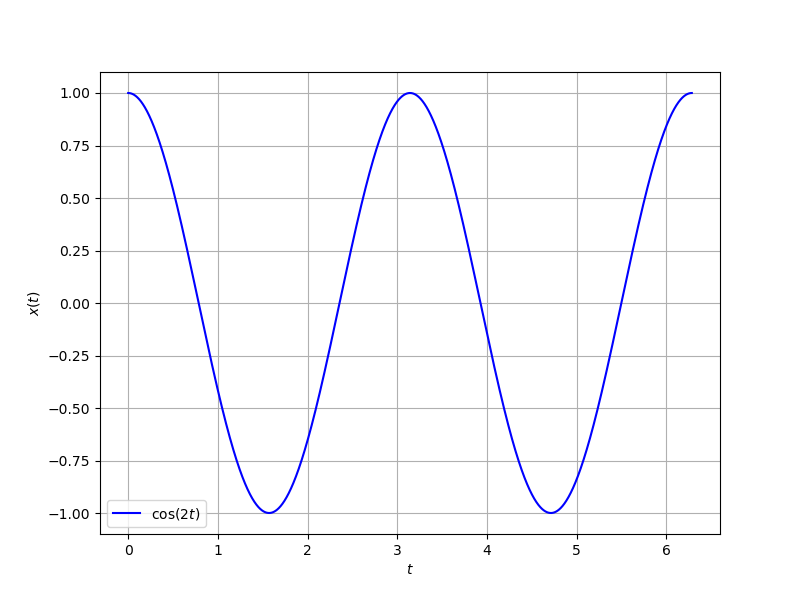
\includegraphics[width=1\linewidth]{2023/EC/35/figs/gate.png}
    \caption{ }
\end{figure}
\solution
\input{2023/EC/35/assign3.tex}
\pagebreak
\item A signal $x\brak{t}=2\cos{(180\pi t)}\cos{(60\pi t)}$ is sampled at 200 Hz and then passed through an ideal low pass filter having cut-off frequency of 100 Hz.\\
The maximum Frequency present in the filtered  signal in Hz is \rule{1cm}{0.5mm} (Round off to the nearest integer.) \hfill (GATE 2023 EE)
\solution
\iffalse
\let\negmedspace\undefined
\let\negthickspace\undefined
\documentclass[journal,12pt,twocolumn]{IEEEtran}
\usepackage{cite}
\usepackage{amsmath,amssymb,amsfonts}
\usepackage{graphicx}
\usepackage{textcomp}
\usepackage{xcolor}
\usepackage{txfonts}
\usepackage{listings}
\usepackage{enumitem}
\usepackage{mathtools}
\usepackage{gensymb}
\usepackage{comment}
\usepackage[breaklinks=true]{hyperref}
\usepackage{tkz-euclide} 
\usepackage{listings}
\usepackage{gvv}                                        
\def\inputGnumericTable{}                                 
\usepackage[latin1]{inputenc}                                
\usepackage{color}                                            
\usepackage{array}                                            
\usepackage{longtable}                                       
\usepackage{calc}                                             
\usepackage{multirow}                                         
\usepackage{hhline}                                           
\usepackage{ifthen}                                           
\usepackage{lscape}
\usepackage[export]{adjustbox}
\usepackage{pgfplots}
\newtheorem{theorem}{Theorem}[section]
\newtheorem{problem}{Problem}
\newtheorem{proposition}{Proposition}[section]
\newtheorem{lemma}{Lemma}[section]
\newtheorem{corollary}[theorem]{Corollary}
\newtheorem{example}{Example}[section]
\newtheorem{definition}[problem]{Definition}
\newcommand{\BEQA}{\begin{eqnarray}}
	\newcommand{\EEQA}{\end{eqnarray}}
\newcommand{\define}{\stackrel{\triangle}{=}}
\newtheorem{rem}{Remark}

\begin{document}
	\parindent 0px
	\bibliographystyle{IEEEtran}
	
	\vspace{3cm}
	
	\title{GATE:EE/63}
	\author{EE23BTECH11208 - Manohar K$^{*}$
	}
	\maketitle
	\newpage
	\bigskip
	
	% \renewcommand{\thefigure}{\theenumi}
	% \renewcommand{\thetable}{\theenumi}
	
	
	
	\textbf{Question:} \hspace{2pt} A signal $x\brak{t}=2\cos{(180\pi t)}\cos{(60\pi t)}$ is sampled at 200 Hz and then passed through an ideal low pass filter having cut-off frequency of 100 Hz.\\
	The maximum Frequency present in the filtered  signal in Hz is \rule{1cm}{0.5mm} (Round off to the nearest integer.) \hfill (GATE 2023 EE)\\
	\noindent \textbf{Solution:}\\
\fi
	\begin{figure}[ht]
		\centering
		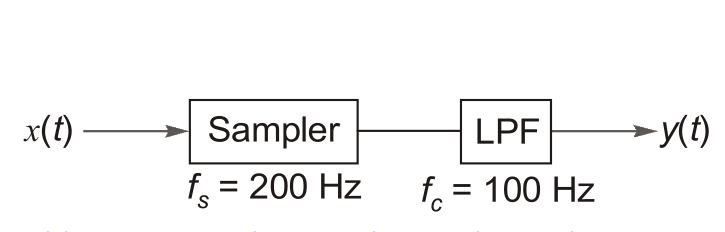
\includegraphics[width=1\linewidth]{2023/EE/63/figs/answerdia.png}
	\end{figure}
	Given, \\
	
	\begin{align}
		x\brak{t}&=\cos\brak{240\pi t} + \cos\brak{120\pi t}
	\end{align}\\
	\begin{table}[h]
		\centering
		
\begin{tabular}{|c|c|c|}
	\hline
	\textbf{symbol} & \textbf{value} & \textbf{description} \\
	\hline
	$x(t)$ & $2\cos{(180\pi t)}\cos{(60\pi t)}$ & input signal \\
	\hline
	$f_s$ & $200Hz$ & sampling frequency \\
	\hline
	$f_c$ & $100Hz$ & cut-off frequency \\
	\hline
	$y(t)$ &  & output signal \\
	\hline
	$f_1$ & $120Hz$ & first signal frequency \\
	\hline
	$f_2$ & $60Hz$ & second signal frequency \\
	\hline
\end{tabular}

		\caption{Parameters}
		\label{tab:GATE.EE.2023.63}
	\end{table}\\
	Aliased frequencies when $f_1$ frequency signal is sampled at $200Hz$\\
	\begin{align}
		& f_1 , \abs{f_s\pm f_1} , \abs{2f_s \pm f_1} \dots\\
		& 120, 80,340,280,520 \dots
	\end{align}
	Aliased frequencies when $f_2$ frequency signal is sampled at $200Hz$\\
	\begin{align}
		& f_2 , \abs{f_s\pm f_2} , \abs{2f_s\pm f_2} \dots\\
		& 60 , 140,260,340,460 \dots 
	\end{align}
\begin{figure}
	\centering
	\begin{tikzpicture}
\begin{axis}[
    axis lines=middle,
    xlabel=$f$,
    ylabel=$X(f)$,
    ymax=1,
    ymin=0,
    xmin=-240,
    xmax=240,
    xtick={ -120, -60, 60, 120},
    ytick={0,1},
    yticklabels={0,1},
    ticklabel style={font=\tiny},
    enlargelimits={abs=0.2},
    clip=false
]
% One-sided arrows
\draw[->, >=latex, blue, thick] (axis cs: -120, 0) -- (axis cs: -120, 1);
\draw[->, >=latex, blue, thick] (axis cs: -60, 0) -- (axis cs: -60, 1);
\draw[->, >=latex, blue, thick] (axis cs: 60, 0) -- (axis cs: 60, 1);
\draw[->, >=latex, blue, thick] (axis cs: 120, 0) -- (axis cs: 120, 1);
\end{axis}
\end{tikzpicture}

	\caption{delta function of input signal }
\end{figure}\\
	
	
\begin{figure}
	\centering
	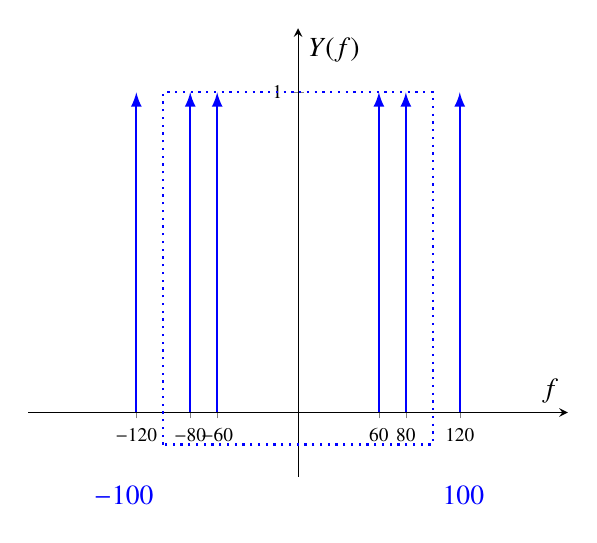
\begin{tikzpicture}
\begin{axis}[
    axis lines=middle,
    xlabel=$f$,
    ylabel=$Y(f)$,
    ymax=1,
    ymin=0,
    xmin=-200,
    xmax=200,
    xtick={ -120, -80, -60, 60, 80, 120},
    ytick={0,1},
    yticklabels={0,1},
    ticklabel style={font=\scriptsize},
    enlargelimits={abs=0.2},
    clip=false
]
% One-sided arrows
\draw[->, >=latex, blue, thick] (axis cs: -120, 0) -- (axis cs: -120, 1);
\draw[->, >=latex, blue, thick] (axis cs: -80, 0) -- (axis cs: -80, 1);
\draw[->, >=latex, blue, thick] (axis cs: -60, 0) -- (axis cs: -60, 1);
\draw[->, >=latex, blue, thick] (axis cs: 60, 0) -- (axis cs: 60, 1);
\draw[->, >=latex, blue, thick] (axis cs: 80, 0) -- (axis cs: 80, 1);
\draw[->, >=latex, blue, thick] (axis cs: 120, 0) -- (axis cs: 120, 1);
% Dotted box
\draw[blue, dotted, thick] (axis cs: -100, -0.1) rectangle (axis cs: 100, 1);
\node[blue, below right] at (axis cs: 100, -0.2) {$100$};
\node[blue, below left] at (axis cs: -100, -0.2) {$-100$};
\end{axis}
\end{tikzpicture}

	\caption{delta function of sampled and filtered signal }
\end{figure}
	from table $f_c = 100Hz$ \\
	LPF output : $60Hz$ , $80Hz$\\
	Maximum Frequency present in the filtered signal is $80Hz$.
	
	
	

\pagebreak
\item In the circuit shown, the input voltage $V_{in} = 100mV$. The switch and the opamp are ideal. At time $t=0$, the intial charge stored in the $10nF$ capacitor is $1nC$, with the polarity as indicated in the figure. The switch $S$ is controlled using a $1KHz$ square-wave voltage signal $V_s$ as shown. Whenever $V_s$ is `High', $S$ is in position $`1$' and when $V_s$ is `Low', $S$ is in position `$2$'.\\
At $t = 20ms$, the magnitude of the voltage $V_o$ will be  \\  
\begin{figure}[ht]
  \centering
    \resizebox{0.55\columnwidth}{!}{\begin{circuitikz}[american]
    \draw (0,0) to[R, l=$10K\Omega$] (2,0) to[L, l=$10mH$] (4,0) to[C, l=$1\mu{F}$] (6,0) -- (6,-1) 
    to[sV, l=$100\cos\brak{\omega_0 t}$] (0,-1) -- (0,0)
    (0,-1) node[circ]{} node[left]{$+$}
    (6,-1) node[circ]{} node[right]{$-$};
\end{circuitikz}
}
\end{figure}
\hfill{(GATE IN 2023)}\\
\solution
\pagebreak

\item The value of parameters of the circuit shown in the figure are $R_1=2\ohm$,$R_2=2\ohm$,$R_3=3\ohm$,$L=10 mH$,$C=100\mu F$. For time \(t<0\), the circuit is at steady state with the switch $ 'K'$ in closed condition. If the switch is opened at $t=0$, the value of the voltage across the inductor \brak{V_L}
 at $t=0^{+}$ in Volts is \rule{2cm}{0.4pt} (Round off to 1 decimal place).
\begin{circuitikz}
    \draw (0,0) to [R, R=$R_3$] (0,2);
    \draw (0,3) to [switch, o-o, name=$K$] (0,2);
    \draw (0,3)-- (0,4);
    \draw (0,4) -- (4,4);
    \draw (3,0) to [american current source, l=$10\,\text{A,}\text{DC}$] (3,4);
    \draw (4,4) to (4,5) to (5,5) to[R, l=$R_1$] (6,5);
    \draw (6,5) to(7,5) to[L, l=$L$] (8,5) to (9,5);
    \draw (4,4)to (4,3)to (5,3) to[R, l=$R_2$] (6,3);
    \draw (6,3)to (7,3) to [C, l=$C$] (8,3) to(9,3);
    \draw (9,5) --(9,3);
    \draw (9,4) -- (10,4);
    \draw (10,4)-- (10,0);
    \draw(10,0)--(0,0);
\end{circuitikz} \hfill (GATE 2023 EE 29Q)
\solution
\pagebreak

\item The op amps in the circuit are ideal. The input signals are $V_{S1} = 3 + 0.10 \sin(300t), \text{V}$ and $V_{S2} = -2 + 0.11 \sin(300t)\, \text{V}$. The average value of the voltage $V_0$ is \underline{\hspace{1cm}} volts (rounded off to two decimal places).
\begin{figure}[ht]
\centering
\resizebox{0.55\columnwidth}{!}{\iffalse
\let\negmedspace\undefined
\let\negthickspace\undefined
\documentclass[a4,12pt,twocolumn]{IEEEtran}
%\documentclass[conference]{IEEEtran}
%\IEEEoverridecommandlockouts
% The preceding line is only needed to identify funding in the first footnote. If that is unneeded, please comment it out.
\usepackage{cite}
\usepackage{amsmath,amssymb,amsfonts,amsthm}
\usepackage{algorithmic}
\usepackage{graphicx}
\usepackage{textcomp}
\usepackage{xcolor}
\usepackage{txfonts}
\usepackage{listings}
\usepackage{enumitem}
\usepackage{mathtools}
\usepackage{gensymb}
\usepackage[breaklinks=true]{hyperref}
\usepackage{tkz-euclide} % loads  TikZ and tkz-base
\usepackage{listings}
\usepackage{empheq}
\usepackage[utf8]{inputenc}
\usepackage{pgfplots}
\usepackage{mathrsfs}
\usepackage{multicol}
\usepackage{array}
%\usepackage{setspace}
%\usepackage{gensymb}
%\doublespacing
%\singlespacing

%\usepackage{graphicx}

\DeclareMathOperator*{\Res}{Res}
%\renewcommand{\baselinestretch}{2}
\renewcommand\thesection{\arabic{section}}
\renewcommand\thesubsection{\thesection.\arabic{subsection}}
\renewcommand\thesubsubsection{\thesubsection.\arabic{subsubsection}}

\renewcommand\thesectiondis{\arabic{section}}
\renewcommand\thesubsectiondis{\thesectiondis.\arabic{subsection}}
\renewcommand\thesubsubsectiondis{\thesubsectiondis.\arabic{subsubsection}}

% correct bad hyphenation here
\hyphenation{op-tical net-works semi-conduc-tor}
\def\inputGnumericTable{}                                 %%

\lstset{
%language=C,
frame=single, 
breaklines=true,
columns=fullflexible
}
%\lstset{
%language=tex,
%frame=single, 
%breaklines=true
%}

\begin{document}
%


\newtheorem{theorem}{Theorem}[section]
\newtheorem{problem}{Problem}
\newtheorem{proposition}{Proposition}[section]
\newtheorem{lemma}{Lemma}[section]
\newtheorem{corollary}[theorem]{Corollary}
\newtheorem{example}{Example}[section]
\newtheorem{definition}[problem]{Definition}
%\newtheorem{thm}{Theorem}[section] 
%\newtheorem{defn}[thm]{Definition}
%\newtheorem{algorithm}{Algorithm}[section]
%\newtheorem{cor}{Corollary}
\newcommand{\BEQA}{\begin{eqnarray}}
\newcommand{\EEQA}{\end{eqnarray}}
\newcommand{\define}{\stackrel{\triangle}{=}}

\bibliographystyle{IEEEtran}
%\bibliographystyle{ieeetr}


\providecommand{\mbf}{\mathbf}
\providecommand{\pr}[1]{\ensuremath{\Pr\left(#1\right)}}
\providecommand{\qfunc}[1]{\ensuremath{Q\left(#1\right)}}
\providecommand{\sbrak}[1]{\ensuremath{{}\left[#1\right]}}
\providecommand{\lsbrak}[1]{\ensuremath{{}\left[#1\right.}}
\providecommand{\rsbrak}[1]{\ensuremath{{}\left.#1\right]}}
\providecommand{\brak}[1]{\ensuremath{\left(#1\right)}}
\providecommand{\lbrak}[1]{\ensuremath{\left(#1\right.}}
\providecommand{\rbrak}[1]{\ensuremath{\left.#1\right)}}
\providecommand{\cbrak}[1]{\ensuremath{\left\{#1\right\}}}
\providecommand{\lcbrak}[1]{\ensuremath{\left\{#1\right.}}
\providecommand{\rcbrak}[1]{\ensuremath{\left.#1\right\}}}
\theoremstyle{remark}
\newtheorem{rem}{Remark}
\newcommand{\sgn}{\mathop{\mathrm{sgn}}}
%\providecommand{\abs}[1]{\left\vert#1\right\vert}
\providecommand{\res}[1]{\Res\displaylimits_{#1}} 
%\providecommand{\norm}[1]{\left\lVert#1\right\rVert}
%\providecommand{\norm}[1]{\lVert#1\rVert}
\providecommand{\mtx}[1]{\mathbf{#1}}
%\providecommand{\mean}[1]{E\left[ #1 \right]}
\providecommand{\fourier}{\overset{\mathcal{F}}{ \rightleftharpoons}}
%\providecommand{\hilbert}{\overset{\mathcal{H}}{ \rightleftharpoons}}
\providecommand{\system}{\overset{\mathcal{H}}{ \longleftrightarrow}}
	%\newcommand{\solution}[2]{\textbf{Solution:}{#1}}
\newcommand{\solution}{\noindent \textbf{Solution: }}
\newcommand{\cosec}{\,\text{cosec}\,}
\providecommand{\dec}[2]{\ensuremath{\overset{#1}{\underset{#2}{\gtrless}}}}
\newcommand{\myvec}[1]{\ensuremath{\begin{pmatrix}#1\end{pmatrix}}}
\newcommand{\mydet}[1]{\ensuremath{\begin{vmatrix}#1\end{vmatrix}}}
%\numberwithin{equation}{section}
%\numberwithin{equation}{subsection}
%\numberwithin{problem}{section}
%\numberwithin{definition}{section}
%\makeatletter
%\@addtoreset{figure}{problem}
%\makeatother

%\let\StandardTheFigure\thefigure
\let\vec\mathbf

\title{
\Huge\textbf{Gate EE 2023}\\
\Huge\textbf{EE1205} Signals and Systems\\
}
\large\author{Nimal Sreekumar\\EE23BTECH11044}

% make the title area
\maketitle


%\tableofcontents

\bigskip

\renewcommand{\thefigure}{\arabic{figure}}
\renewcommand{\thetable}{\theenumi}
%\renewcommand{\theequation}{\theenumi}


\textbf{Question Gate 2023 EE:}
For the signals x\brak{t} and y\brak{t} shown in the figure, $z\brak{t}=x\brak{t}*y\brak{t}$ is maximum at $t=T_1$. Then $T_1$ in seconds is .......... \brak{\text{Round off to the nearest integer}}\\

\begin{tikzpicture}
\begin{axis}[xmin=-3, xmax=7, ymin=-3, ymax=3, axis lines=middle, xlabel={$t$}, title={$y\brak{t}$}]
 \addplot[blue] coordinates {(-3,0) (1,0)};
  \addplot[blue] coordinates {(1,0) (1,-2)};
   \addplot[dashed] coordinates {(0,-2) (1,-2)};
  \addplot[blue, domain=1:5] {x - 3};
  \addplot[blue] coordinates {(5,2) (5,0)};
  \addplot[blue] coordinates {(5,0) (7,0)};
  \addplot[dashed] coordinates {(0,2) (5,2)};
    \end{axis}
\end{tikzpicture}

\begin{tikzpicture}
    \begin{axis}[xmin=-3, xmax=3, ymin=-3, ymax=3, axis lines=middle, xlabel={$t$} ,title={$x\brak{t}$}]
        \addplot[blue] coordinates {(-3,0) (-1,0)};
        \addplot[blue] coordinates {(-1,0) (-1,1)};
        \addplot[blue] coordinates {(-1,1) (1,1)};
        \addplot[blue] coordinates {(1,1) (1,0)};
        \addplot[blue] coordinates {(1,0) (3,0)};
    \end{axis}
\end{tikzpicture}

\hfill (GATE EE 2023)
\solution
\fi

\begin{table}[htbp]
\centering
\renewcommand\thetable{1}
\begin{tabular}{|c|m{3.5cm}|m{3cm}|}
    \hline
    \textbf{Variable} & \textbf{values} & \textbf{Description} \\
    \hline
    $x\brak{t}$ & $u\brak{t+1}-u\brak{t-1}$ & signal 1\\
    \hline
    $ y\brak{t} $ & $y\brak{t} = 
    \begin{cases}
        t-3 & ; 1\leq n \leq 5 \\
        0 & ; otherwise \\
    \end{cases}$ & signal 2\\
    \hline
    $X\brak{s}$ & $\int_{0}^{\infty}x\brak{t}e^{-st}dt$ & Laplace transform of $x\brak{t}$\\
    \hline
   $Y\brak{s}$ & $\int_{0}^{\infty}y\brak{t}e^{-st}dt$ & Laplace transform of $y\brak{t}$ \\
    \hline
    $\mathscr{L^{-1}} \{Z(s)\}$ &$f\brak{t-c}u\brak{t-c}=\mathscr{L^{-1}}\brak{e^{-cs}F\brak{s}} $& Inverse Laplace transform \\
    \hline
\end{tabular}
\caption{Input Parameters}
\label{tab:11.9.5.32}
\end{table}

Using laplace transform,
\begin{align}
z\brak{t} &=x\brak{t}*y\brak{t}\label{eq:gate_ee_Q31.1} \\
Z\brak{s} &=X\brak{s}Y\brak{s}\label{eq:gate_ee_Q31.2} \\
X\brak{s} &= \frac{1}{s} \brak{e^{s}-e^{-s}} \label{eq:gate_ee_Q31.3}\\
Y\brak{s} &= \frac{2s+1}{s^2} \brak{e^{-s}-e^{-5s}}\label{eq:gate_ee_Q31.4}\\
Z\brak{s} &= \frac{2s+1}{s^3} \brak{1-e^{-4s}-e^{-2s}+e^{-6s}}\label{eq:gate_ee_Q31.5}
\end{align}
Now taking inverse laplace transform for each terms, $\mathscr{L^{-1}} \{Z(s)\}$
\begin{align}
&= \left( 2t + \frac{t^2}{2} \right) u(t) \nonumber \\
&\quad - \left( 2(t-4) + \frac{(t-4)^2}{2} \right)u(t-4) \nonumber \\
&\quad - \left( 2(t-2) + \frac{(t-2)^2}{2} \right)u(t-2) \nonumber \\
&\quad + \left( 2(t-6) + \frac{(t-6)^2}{2} \right)u(t-6) \nonumber
\end{align}\label{eq:gate_ee_Q31.6}
From the plot it is clear that $T_1=4$.\\
\begin{figure}[h]
\centering
   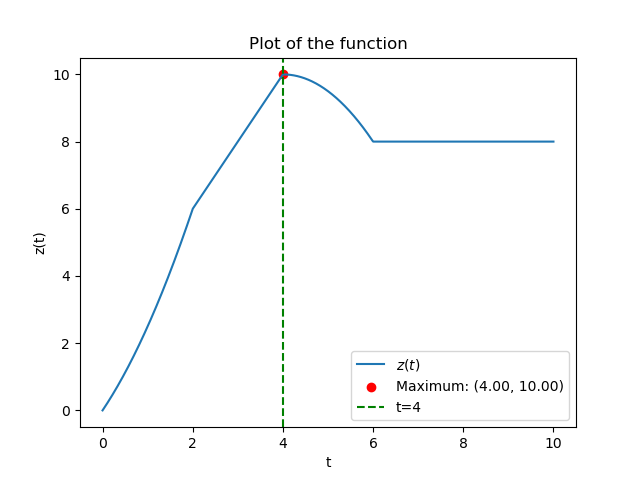
\includegraphics[width=1\linewidth]{2023/EE/31/figs/figs/gate2023EE.png}
   \caption{z\brak{t} vs. t}
   \label{fig:gate2023EE1}
 \end{figure}\\
Now in time domain,
 \begin{align}
z\brak{t} &=x\brak{t}*y\brak{t} = y\brak{t}*x\brak{t}\label{eq:gate_ee_Q31.7}\\
z\brak{t} &=\int_{-\infty}^{\infty} y\brak{\tau}x\brak{t-\tau}d\tau\label{eq:gate_ee_Q31.8}
\end{align}
$x\brak{\tau}$ is an even signal,
\begin{align}
x\brak{\tau}= x\brak{-\tau}\label{eq:gate_ee_Q31.9}\\
 x\brak{-\tau}= 
    \begin{cases}
        1 & ; -1\leq -\tau \leq 1 \\
        0 & ; \text{otherwise} \\
    \end{cases}\label{eq:gate_ee_Q31.10}
    \end{align}
    
    \begin{align}
    x\brak{-\tau} \xleftrightarrow{\text{Time shifting}} x\brak{t-\tau}\label{eq:gate_ee_Q31.11} \\
    x\brak{t-\tau}= 
    \begin{cases}
        1 & ; t-1\leq t-\tau \leq t+1 \\
        0 & ; \text{otherwise} \\
    \end{cases}\label{eq:gate_ee_Q31.12}
\end{align}\\
For $z\brak{t}$ to be maximum both $y\brak{\tau}$ and $x\brak{t-\tau}$ must be maximum,
\begin{align}
\implies t-1 &= 3 \quad \text{or} \quad t+1 = 5 \nonumber \\
t &= T_1 = 4 \nonumber
\end{align}
}
\end{figure}
\hfill{(GATE IN 2023)}

\end{enumerate}
